\documentclass[a4paper,titlepage,12pt]{article}

% NOTE: packages used
\usepackage{geometry}
\usepackage{graphicx}
\usepackage{amssymb}
\usepackage{hyperref}
\usepackage{epstopdf}
\usepackage{color}
\usepackage{xcolor}
\usepackage{xcolor, listings}
\usepackage{caption}
\usepackage{url}
\usepackage{graphicx,pdflscape}
\usepackage[utf8]{inputenc}
\usepackage{listings}
\usepackage{parskip}
% \usepackage{fullpage}
\definecolor{lightgrey}{HTML}{eeeeee}


% NOTE: declarations and definitions document wide:
\DeclareCaptionFormat{listing}{\colorbox{lightgrey}{\parbox{\textwidth}{#1#2#3}}}
\captionsetup[lstlisting]{format=listing}
\DeclareGraphicsRule{.tif}{png}{.png}{`convert #1 `dirname #1`/`basename #1 .tif`.png}

\setlength{\parskip}{0.3in}
\setlength{\parindent}{0in}

% dark green:

\lstloadlanguages{Java}
\lstset{
  % language=Java,
  % morecomment=[s][\color{blue}]{\:}{\ },
  % morecomment=[s][\color{magenta}]{\=\>}{\ },
  basicstyle=\footnotesize,
  tabsize=2,
  breaklines=true,
  breakatwhitespace=true,
  % numberstyle=\tiny,
  % firstnumber=1,
  % basicstyle=\ttfamily\color{black},
  % commentstyle=\ttfamily\color{gray},
  % keywordstyle=\ttfamily\color{red},
  % stringstyle=\color{green},
  % numberstyle=\ttfamily\color{magenta}
}


\title{Comparision of NeoDatis and PostgreSQL.}
\author{\href{mailto:i@teamon.eu}{Tymon Tobolski}}
\date{2011-05-19}


% NOTE: document content:
\begin{document}
\maketitle
\tableofcontents

\section{Introduction}\label{sec:introduction}


The object of research is highly efficient databse system for storing information about UNIX processes. Each couple of seconds processes are sampled and its PID, name, CPU and memory usage is saved into databse along with current timestamp. Measured parameters are time of storage and disk space usage for every database system. On the other hand persisting data is pointless without ability of creating reports out of it, in this case detailed usage for specified time range, PID or name as well as total and average statistics.

The two compared databases are NeoDatis \footnote{Neodatis - \url{http://neodatis.org}} and PostgreSQL\footnote{PostgreSQL - \url{http://postgresql.org}}.

PostgreSQL is an Relational Database Management System (RDBMS) that started over 15 years ago and currently has the position of "The world's most advanced open source database". It has been adopted by many companies and has proven its capatibilities.

NeoDatis is an relatively young Object Oriented Database Management System (OODBMS) that runs on Java Virtual Machine and .NET platforms. It provides very easy and almost transparent persistance layer for object oriented applications. It stores data as objects instead of table records

All test were written in Scala \footnote{Scala language - \url{http://scala-lang.org}} language that runs on top of Java Virtual Machine. While NeoDatis provides object level API, to achieve the same level of abstraction with PostgreSQL an Object Relational Mapper (ORM) library Squeryl \footnote{Squeryl ORM - \url{http://squeryl.org/}} has been used.

In next sections \emph{record} in the context of PostgreSQL will refer to a record in database table, and to a persisted object in the context of NeoDatis.


\section{Benchmark environment}\label{sec:tech_info}

All benchmarks were performed on MacBook Pro running Mac OSX 10.6.7 with 2.4 GHz Intel Core 2 Duo processor and 8 GB of RAM.

\begin{itemize}
    \item Java Virtual Machine
        \begin{lstlisting}[language=bash]
        $ java -version
        java version "1.6.0_24"
        Java(TM) SE Runtime Environment (build 1.6.0_24-b07-334-10M3326)
        Java HotSpot(TM) 64-Bit Server VM (build 19.1-b02-334, mixed mode)
        \end{lstlisting}
        
    \item Scala language version 2.9
    \item NeoDatis ODB version 1.9.30.689
    \item Squeryl library version 0.9.4-RC6
    \item JDBC PostgreSQL driver version 9.0-801.jdbc4
    \item PostgreSQL version 9.0.4 (x86\_64)


\end{itemize}

\section{Batch insert performance}\label{sec:batch_insert}


The most important factor when choosing database management system for described architecture is its ability to perform fast insert of many records in very short time.

The measured value was time of storing 100000 objects devided in parts containing 1, 10, 100, 1,000 or 10,000 items. In order to notice difference and exclude cache from benchmark each part was commited after saving. This opeartion required database transactions, which is enabled in NeoDatis by default and do not require any modifications. Code for PostgreSQL used standard SQL transactions. SQL provides a way of inserting several record within single query, while NeoDatis API lacks this feature. Pseudocode of performed operations is presented below.

\begin{lstlisting}[language=Java, caption=NeoDatis code]
for(obj in objects) {
    odb.store(obj)
}
odb.commit()
\end{lstlisting}

\begin{lstlisting}[language=Java, caption=PostgeSQL code]
psql.saveList(objects) // Performs only single INSERT 
                       // query with multiple values
psql.commit()
\end{lstlisting}



When storing one record at the time (presented as 1x label) NeoDatis performs save much faster than PostgresSQL. However, when part size increases to 10 records PostgreSQL gets about 6x time boost, while NeoDatis with client-server running on the same virtual machine performs 4 times faster and NeoDatis running on separate JVM's is only 1.5 times faster than when saving one record at the time. Increasing part size to 100 provides next big improvement in PostgeSQL storing time (about 4.5x) but hardly any for NeoDatis.
Saving 1000 and 10000 records at one takes aproximately the same amount of time as when saving parts that contain 100 items.

When comparing performance between NeoDatis with client-server running in the same Java runtime and PostgreSQL, NeoDatis saves objects about 1.5x faster than PostgreSQL. However, PostgreSQL server runs in separate process and comunicates with client via network (TCP/IP). Saving data to NeoDatis server using network is much slower (10 times than local NeoDatis and 6 times slower than PostgreSQL).

Benchmark results are presented in Figure \ref{fig:batch_insert}.


\begin{landscape}
    \begin{figure}[p]
        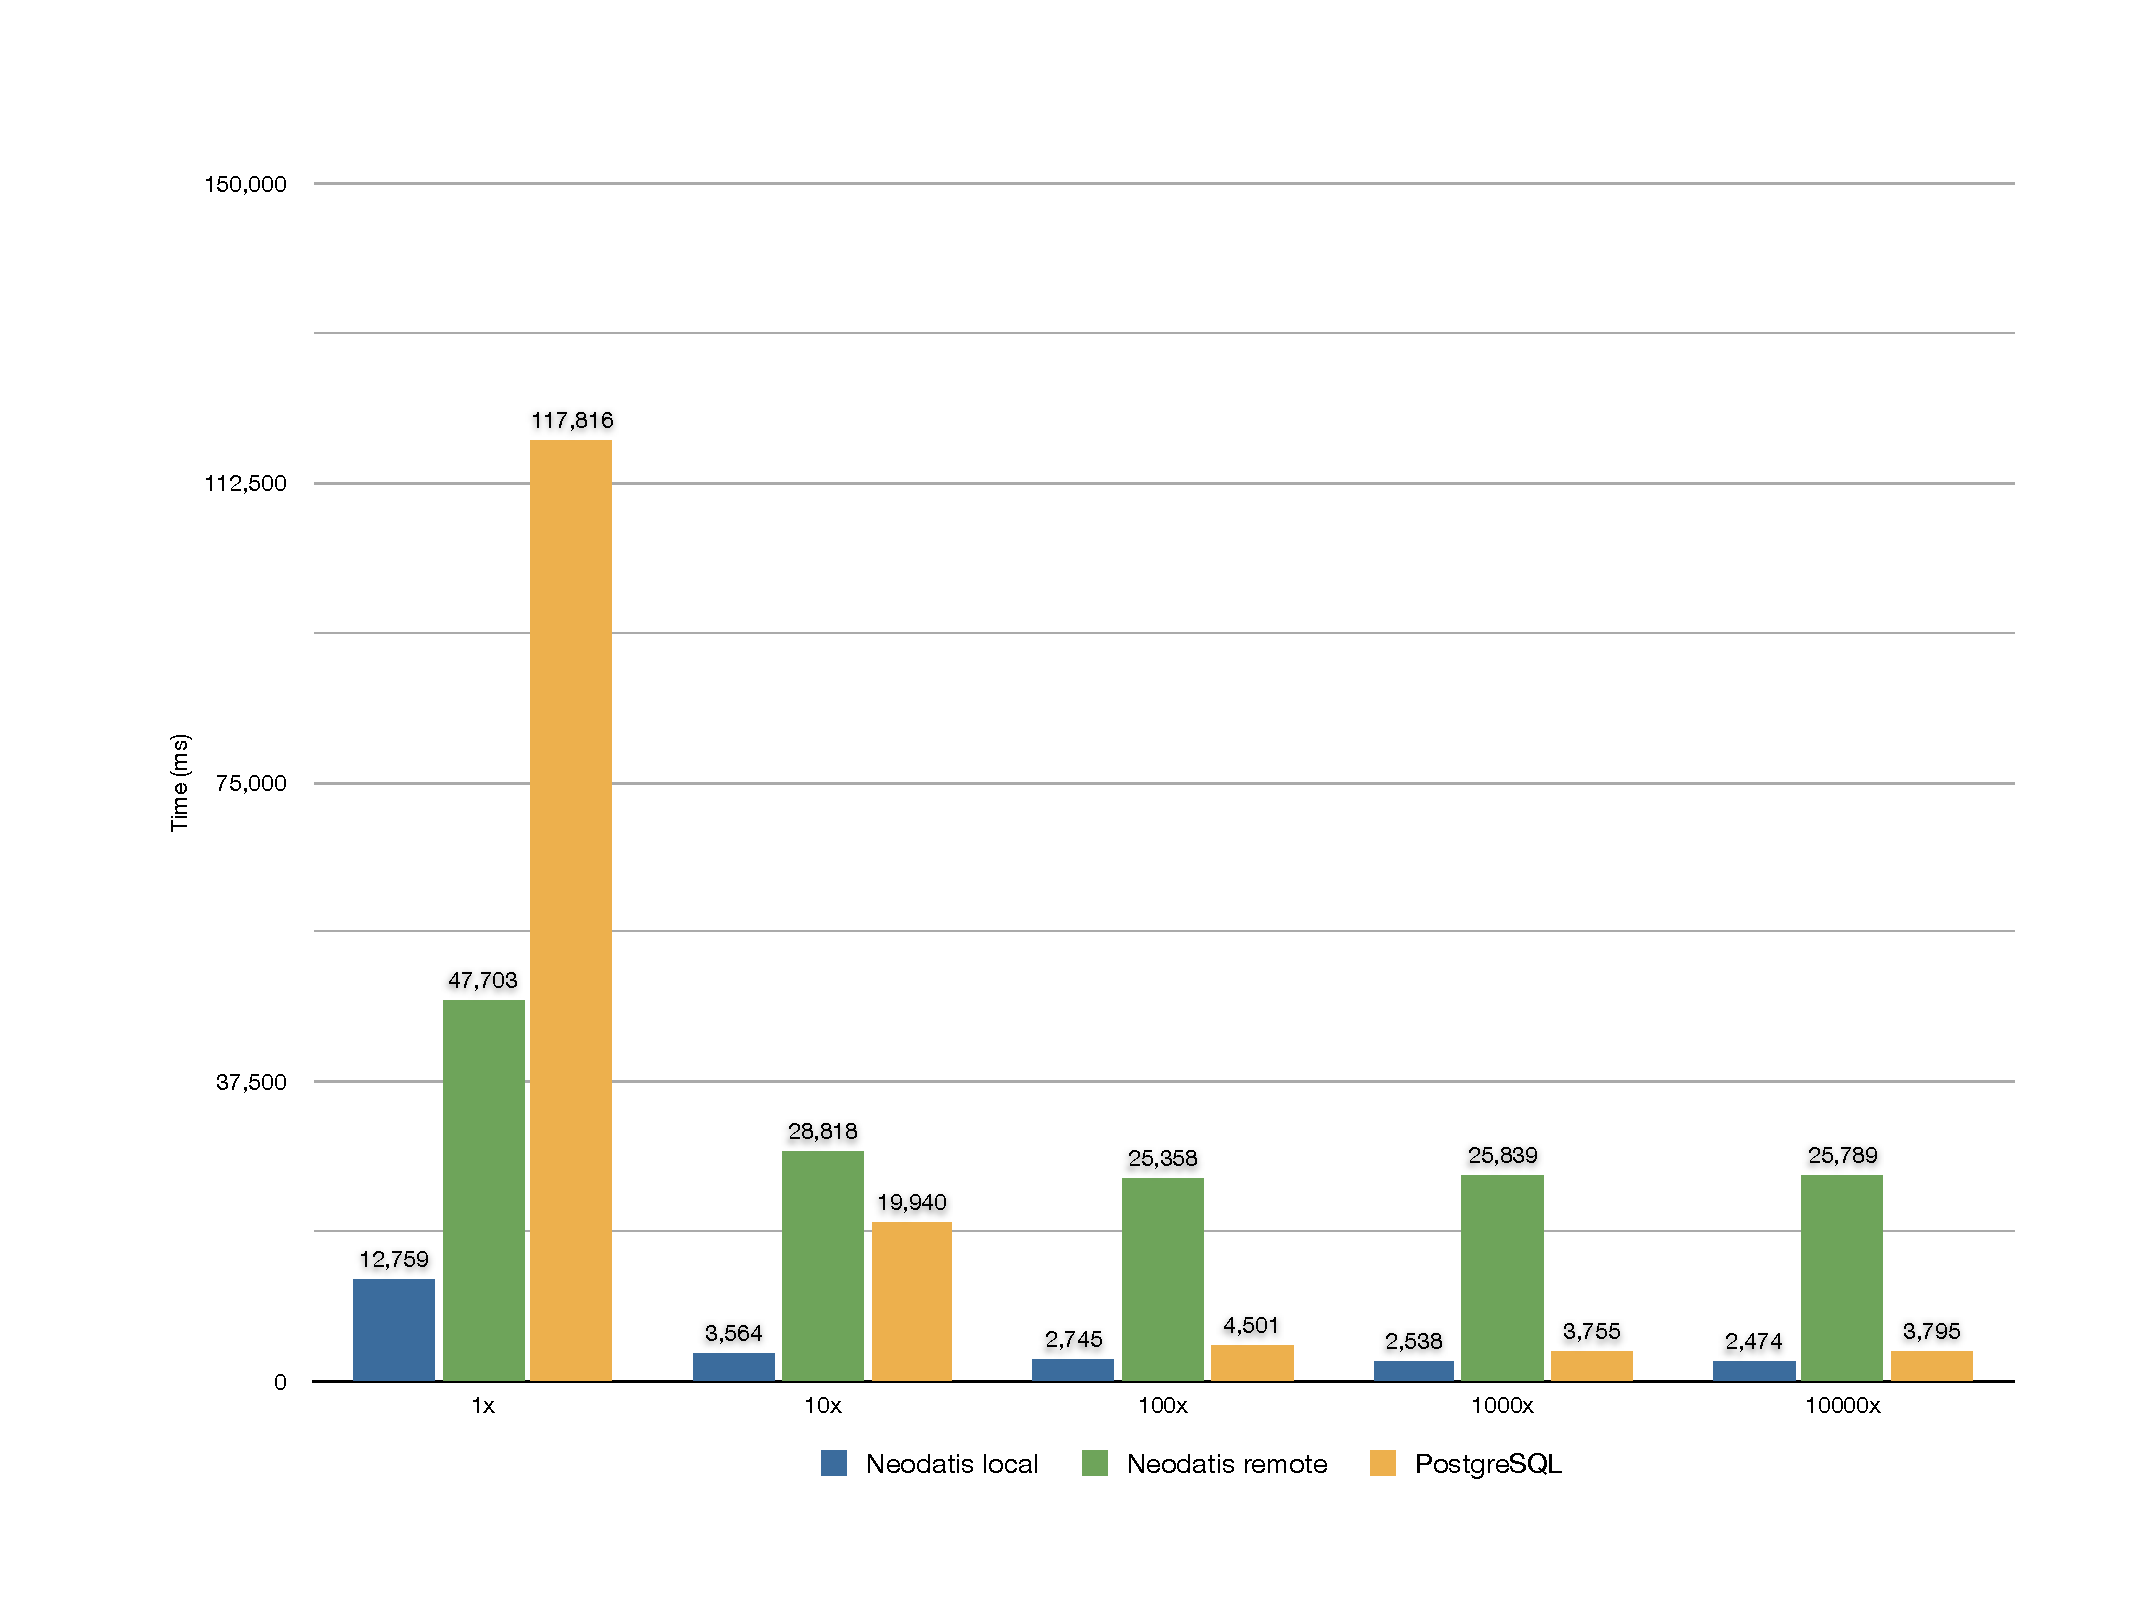
\includegraphics[scale=0.6]{Fig1.pdf}
        \caption{Batch insert speed benchmark}
        \label{fig:batch_insert}
    \end{figure}
\end{landscape}

\section{Query performance}\label{sec:query_performance}

\section{Disk space usage}\label{sec:disk_space_usage}
One of the fundamental parameter of databse management system is disk space usage.
Frequent storing of many objects can quickly fill up disk storage. To compare space used by databases the same amount of exactly identical objects has beed saved using each database. NeoDatis stores each database in separate file, its size was the measured value. PostgreSQL provides SQL function $pg\_database\_size$ which can be executed like:

\begin{lstlisting}[caption=PostgeSQL database size]
SELECT pg_database_size("dbname");
\end{lstlisting}

% Results are presented in Figure \ref{fig:size}

In NeoDatis correlation between number of stored records and database file size is linear. This kind of characteristic provides an easy way of predicting database size for any number of records. Under 1,000,000 of reocrds PostgrSQL has slightly different characteristic, but it becames linear as soon as database size reaches more than 1 million objects. However, in comparision with PostgreSQL NeoDatis uses about 4 times more disk space for 1,000,000 records (NeoDatis uses 218MB while PostgreSQL uses only 55MB) and about 2.7x more for 10,000,000 records (NeoDatis - 2,184MB, PostgreSQL - 795MB).

Detailed results are presented in Figure \ref{fig:size}.


\begin{landscape}
    \begin{figure}[p]
        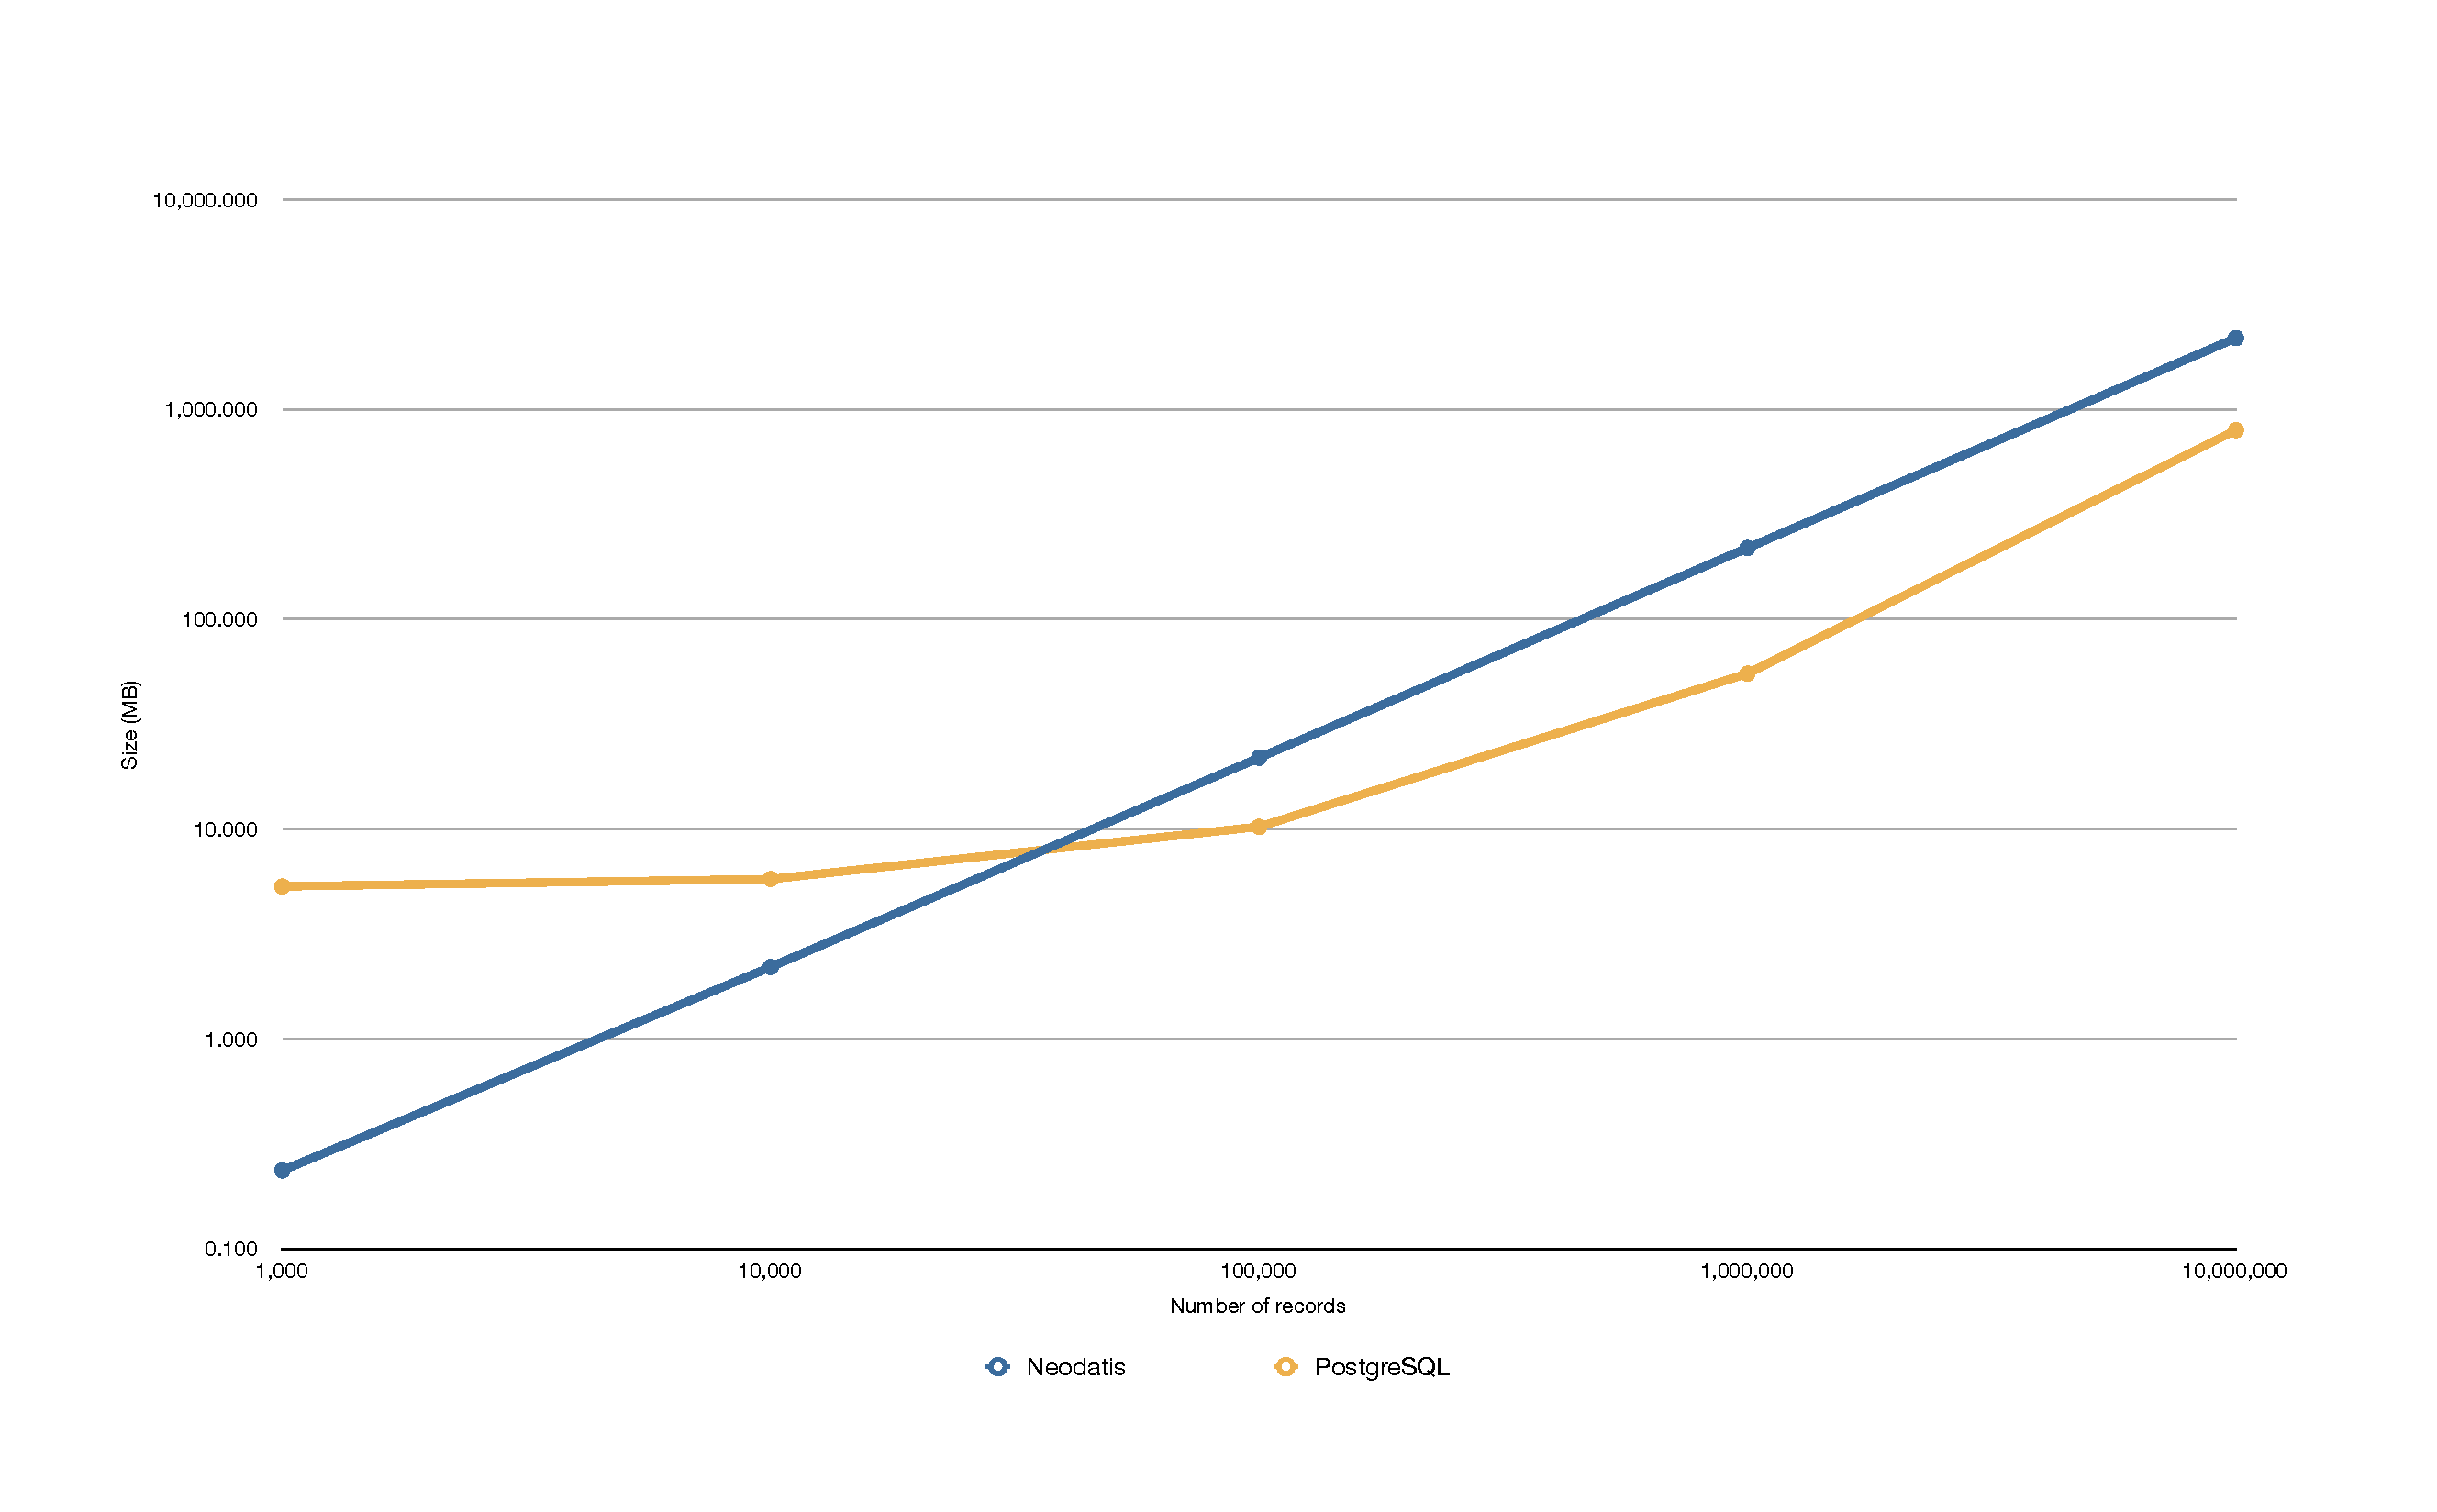
\includegraphics[scale=0.5]{FigSize.pdf}
        \caption{Disk space usage}
        \label{fig:size}
    \end{figure}
\end{landscape}




\end{document}

































% 
% 
%   \subsection{database\_count}\label{sub:database_count}
%     \emph{Script arguments: cluster-name. Default: Master}
%     \\\\Checks defined count of records in defined databases on given cluster-name.
%     
%     
%   \subsection{distributor}\label{sub:distributor}
%     \emph{Script arguments: work-mode cluster-name
%       \\work-mode - normal or critical. Default mode: none.
%       \\cluster-name - choose from which database definition, dump list should be taken from. If undefined dump list in backup cluster config, then Master cluster settings will be used. Default cluster: backup}
%     \\\\Sends database dumps to remote destinations (S3/FTP).
%     Critical mode will also automatically include all SQL dumps available/ defined in cluster configuration.
%   
% 
%   \subsection{file\_dump}\label{sub:file_dump}
%     \emph{Script arguments: work-mode
%       \\work-mode - normal or critical. Default mode: none}
%     \\\\Synchronizes current user files defined in config to ``\hyperref[sub:backup_live]{backup\_live}'' folder, from which \hyperref[sub:distributor]{distributor} is taking files for remote backup.
%     
%     
%   \subsection{maintenance}\label{sub:maintenance}
%     \emph{Script arguments: action database-name cluster-name
%       \\action - currently one of: vacuum\_full, vacuum\_analyze, vacuum, reindex\_table, reindex, reindex\_database, reindex\_system.
%       \\database-name - database to perform action on. Default database: none
%       \\cluster-name - cluster to perform action on. Default cluster: Master}
%     \\\\Performs various actions on given database in given cluster. Currently only vacuum* and reindex* actions are defined.
%   
%   
%   \subsection{replicator}\label{sub:replicator}
%     \emph{Script arguments: behaviour
%       \\behaviour - one of: scratch, normal, standalone, stopall, failover, status}
%     \\\\Depending on behaviour, given script will perform predefined actions:
%     \begin{itemize}
%       \item scratch - will stop and destroy all defined clusters, afterwards recreate all of them from scratch, rebuild all databases from sql dumps, and start both standalone clusters and replication mode for defined Master/Slave clusters. After this task is done, whole database is production ready.
%       \item normal - will stop all Master/Slave/Standalone clusters defined in config, afterwards will start replication mode for defined Master/slaves and restart standalone clusters. This action is non-destructive. After this task is done, whole database is production ready (if clusters aren't corrupted or misconfigured)
%       \item standalone - will restart standalone clusters defined in config. Master and Slaves wont be touched.
%       \item stopall - will stop all clusters defined in config. This includes Master, Slaves and Standalones.
%       \item status - prints currently running postgres nodes.
%       \item failover - currently unimplemented yet
%     \end{itemize}
%     
%   
%   \subsection{restore}\label{sub:restore}
%     \emph{Script arguments: cluster-name}
%     \\\\Performs recreation of given cluster from scratch, and recreates all defined databases from config. This will permanently destroy all data of given cluster.
%     
%     
%   \subsection{s3compactor}\label{sub:s3compactor}
%     \emph{Script arguments: none}
%     \\\\Performs automatic process of compaction of dumps and files on remote S3 cloud storage.
%     
%     
%   \subsection{s3get}\label{sub:s3get}
%     \emph{Script arguments: regexp-pattern}
%     \\\\Performs checkout on remote S3 dumps for files matching given regexp-pattern.
%     
%   
%   \subsection{s3send}\label{sub:s3send}
%     \emph{Script arguments: file-to-send [file-prefix]
%       \\file-to-send - file to be send
%       \\file-prefix - optional prefix prepended to file before sending to remote backup host. Default: date-time defined in config}
%     \\\\Sends given file-to-send file (path to file should be absolute) to defined remote backup destinations (S3/FTP).
%     
%   
%   \subsection{sql\_dump}\label{sub:sql_dump}
%     \emph{Script arguments: cluster-name
%       \\cluster-name - defined cluster name from which SQL database dump will be performed. Master cluster is not allowed here}
%     \\\\Performs SQL database dump from given cluster. If cluster is defined as Slave, then it will stop Slave connection with Master afterwards turn off replication process, perform SQL dump, resync database files from Master through rsync and restarts replication process and connection with Master.
%     \\If cluster is defined as Standalone, it will just perfom dump and nothing more.
%   
%   
%   \subsection{sysconfig}\label{sub:sysconfig}
%     \emph{Script arguments: none}
%     \\\\This is the only one script which currently requires root privileges to run. Currently it prepares rsync configuration. Requires single run on each host.
%     
%     
% 
% \section{Config values explanation (What-is-What)}\label{sec:whatiswhat}
%   
%   
%   \subsection{PostgreSQL related settings}\label{sub:postgres}
%     \begin{itemize}
%       \item REPLICATION\_STRUCTURE\_MAP - main map contains general cluster configuration of PSQL clusters
%         \begin{lstlisting}[caption=Master cluster definition]
% "master-cluster-name" => {
%   :mode => :master, # only one master entry allowed
%   :ip => "HOSTNAME", # by default 127.0.0.1
%   :login => DEFAULT_USER, # default system user
%   :port => 65432, # unique port number
%   # wal_destination is required for master cluster
%   :wal_destination => "/srv/psql-wal-folder",
%   # conf_dir, data_dir, log_dir may point same directory
%   :conf_dir => "/srv/unique-psql-conf-dir", # postgresql.conf
%   :data_dir => "/srv/unique-psql-data-dir", # data directory
%   :log_dir => "/srv/unique-psql-log-dir", # log directory
%   :roles => [ # array of roles for given cluster
%     ["login-role", "login-password"],
%   ],
%   :databases => { # databases defined in cluster
%     # database name => database owner
%     "database-name" => "default-database-owner",
%   },
%   :requirements => { # requirements for database
%     "database-name" => {
%       10000 => %w(table1 table2 table3),
%       1000 => %w(table4 table5 table6),
%       100 => %w(tableX tableY tableZ),
%       10 => %w() # minimum record count => tables
%     },
%   }
% },
%         \end{lstlisting}
% 
%         \begin{lstlisting}[caption=Slave clusters definition]
% # some slave
% "slave" => {
%   :mode => :slave, # multiple slaves allowed
%   :ip => "HOSTNAME", # by default 127.0.0.1
%   :login => DEFAULT_USER, # default system user
%   :port => 65433, # unique port number
%   # conf_dir, data_dir, log_dir may point same directory
%   :conf_dir => "/srv/unique-psql-conf-dir",
%   :data_dir => "/srv/unique-psql-data-dir",
%   :log_dir => "/srv/unique-psql-log-dir",
% },
% 
% # slave used by default by sql_dumper
% "backup" => {
%   :mode => :slave,
%   :ip => "HOSTNAME", # by default 127.0.0.1
%   :login => DEFAULT_USER, # default system user
%   :port => 65434, # unique port number
%   # conf_dir, data_dir, log_dir may point same directory
%   :conf_dir => "/srv/unique-psql-conf-dir",
%   :data_dir => "/srv/unique-psql-data-dir",
%   :log_dir => "/srv/unique-psql-log-dir",
% },
%         \end{lstlisting}
% 
%         \begin{lstlisting}[caption=Standalone clusters definition]
% # standalones:
% "standalone-devel1" => {
%   :mode => :standalone,
%   :ip => "HOSTNAME", # by default 127.0.0.1
%   :login => DEFAULT_USER, # default system user
%   :port => 65435, # unique port number
%   :roles => [ # array of roles for given cluster
%     ["role1", "password-role1"],
%   ],
%   :databases => { # databases defined in cluster
%     # database name => database owner
%     "database_name" => "role1"
%   },
%   # conf_dir, data_dir, log_dir may point same directory
%   :conf_dir => "/srv/unique-psql-conf-dir",
%   :data_dir => "/srv/unique-psql-data-dir",
%   :log_dir => "/srv/unique-psql-log-dir",
% },        
%         \end{lstlisting}
%       
%     \end{itemize}
%     
%       
%   \subsection{AmazonS3/FTP and backup related settings}\label{sub:backup}
%     \begin{itemize}
%       \item AMAZON\_AUTH - definition of Amazon S3 authorization
%       \begin{lstlisting}[caption=Amazon S3 configuration]
% AMAZON_AUTH = {
%   :access_key_id => 'S3_ACCESS_ID', # empty access_key_id will cause sending to be skipped.
%   :secret_access_key => 'S3_ACCESS_KEY',
%   :bucket => "BackupD-#{Time.now.year}", # name of default bucket to upload files to
%   :keep_days => 90 # amount of days to keep S3 dumps. Used by s3compactor.
% }
%       \end{lstlisting}
%       \item FTP\_AUTH - definition of FTP authorization
%       \begin{lstlisting}[caption=FTP configuration]
% FTP_AUTH = {
%   :host => 'FTP_HOST', # empty host will cause sending to be skipped
%   :user => 'FTP_USER_NAME',
%   :password => 'FTP_USER_PASSWORD'
% }
%       \end{lstlisting}
%     \end{itemize}
%   
%   \subsection{System, Command related settings}\label{sub:system}
%     \begin{itemize}
%       \item SYSTEM\_ACCESS\_KEYS\label{sub:system_access_keys} - array of SSH-RSA public keys used by system users to log in to system.
%       \item DIRECTORIES\label{sub:directories} - includes :normal and :critical directories defined for synchronization to ``\hyperref[sub:backup_live]{backup\_live}'' directory (\hyperref[sub:file_dump]{file\_dump} and \hyperref[sub:sql_dump]{sql\_dumper}).
%       \begin{lstlisting}[caption=Directories which will be synchronized by rsync to local  ``backup\_live'']
% DIRECTORIES = {
%   :normal => [
%     "/srv/home/someuser/something/somewhere",
%     "/srv/home/anotheruser/anything/here",
%   ],
%   :critical => [
%     "/srv/home/infakt/git",
%   ]
% }
%       \end{lstlisting}
%       \item DISTRIBUTION\label{sub:distribution} - List of files used by \hyperref[sub:distributor]{distributor}. All taken from ``\hyperref[sub:backup_live]{backup\_live}'' directory.
%       \begin{lstlisting}[caption=List of directories that will be distributed to remote S3/FTP]
% DISTRIBUTION = {
%   :normal => [
%     BACKUP_LIVE_DIRECTORY_FS + "somewhere",
%   ],
%   :critical => [
%     BACKUP_LIVE_DIRECTORY_FS + "here",
%   ]
% }
%       \end{lstlisting}
%       \item BACKUP\_LIVE\_DIRECTORY\_FS\label{sub:backup_live} - directory to which \hyperref[sub:directories]{DIRECTORIES} are synchronized to by \hyperref[sub:file_dump]{file\_dump}. These are raw copy of files defined in \hyperref[sub:directories]{DIRECTORIES} constant.
%       \item BACKUP\_LIVE\_DIRECTORY\_DUMPS - directory in which all defined SQL dumps are collected to.
%     \end{itemize}
%   
% \end{document}
% 

